\chapter{1er lancement}
Au premier d\'emarrage du logiciel, une fen\^etre de configuration se lance.
Elle se compose d'une fen\^etre de << Bienvenue >>, d'une de configuration de la base de donn\'ees et d'une de saisi de vos informations personnelles.

\begin{figure}[H]
	\centering
	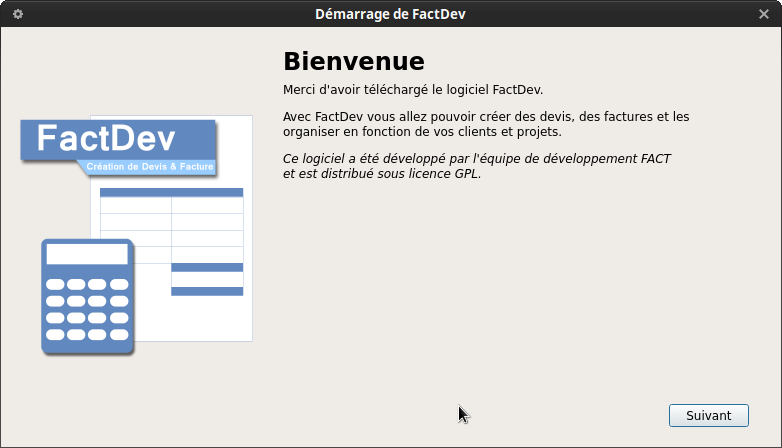
\includegraphics[width=12cm]{screens/lancement1.png}
	\caption{Premier lancement de FactDev}
	\label{fig:lancementFactDev}
\end{figure}

\section{Configuration de la base de donn\'ees}
Dans ces partie il faut choisir entre deux types de base de donn\'ees comme le montre les images ci-dessous.
\begin{figure}[H]
	\centering
	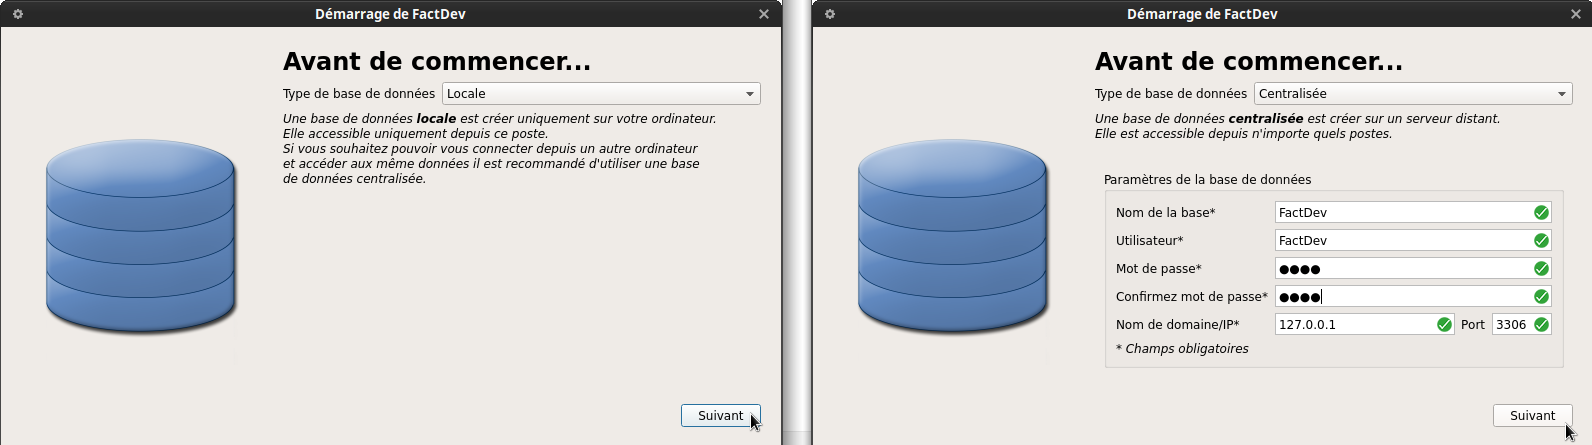
\includegraphics[width=15cm]{screens/lancement2.png}
	\caption{Configuration de la base de donn\'ees}
	\label{fig:configurationBaseDeDonnees}
\end{figure}
Le type de base de donn\'ees \textbf{locale} indique que les donn\'ees sont stock\'ees uniquement sur votre ordinateur. Vous aurez donc acc\`es \`a ces informations uniquement depuis ce poste. 

La base de donn\'ees \textbf{centralis\'ee} est cr\'e\'ee sur un serveur distant. Cela signifie que, d\`es lors que l'on dispose d'une connexion internet, on peut acc\'eder aux donn\'ees du logiciel quelque soit l'ordinateur que l'on utilise. 
Dans ce dernier cas, des champs doivent \^etre renseign\'es: \\
\begin{description}
	\item[Nom de la base] (Obligatoire) Nom de la base de donn\'ees (FactDev par d\'efaut)
	\item[Utilisateur] (Obligatoire) Pseudonyme de l'utilisateur du logiciel (FactDev par d\'efaut)
	\item[Mot de passe] (Obligatoire) Mot de passe de l'utilisateur
	\item[Confirmez Mot de passe] (Obligatoire) V\'erifie que l'utilisateur a correctement saisi son mot de passe
	\item[Nom de domaine/IP] (Obligatoire) Nom de domaine du serveur distant ou son adresse IP (127.0.0.1 par d\'efaut)
	\item[Port] Num\'ero de port du serveur (3306 par d\'efaut)
\end{description} 

\section{Informations vous concernant}
La derni\`ere \'etape consiste \`a renseigner les informations de votre entreprise. 
\begin{figure}[H]
	\centering
	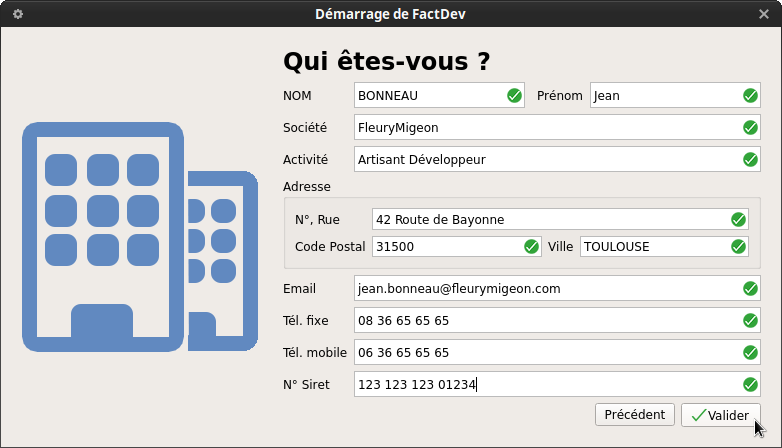
\includegraphics[width=12cm]{screens/lancement3.png}
	\caption{Renseignement des informations de l'entreprise}
	\label{fig:renseignementInformationsEntreprise}
\end{figure}
Les informations \`a renseigner sont:
\begin{description}
	\item[NOM] (Obligatoire) Votre NOM de famille
	\item[Pr\'enom] (Obligatoire) Votre pr\'enom
	\item[Soci\'et\'e] (Obligatoire) Le nom de votre soci\'et\'e
	\item[Activit\'e] Activit\'e de votre entreprise, slogan ou message qui la caract\'erise
	\item[Adresse] (Obligatoire) Adresse \`a laquelle se trouve votre entreprise
	\item[Email] (Obligatoire) Votre adresse e-mail professionnelle
	\item[T\'el\'ephone/Fax] Num\'ero de t\'el\'ephone (fixe ou mobile) et Fax. L'un des deux num\'eros de t\'el\'ephones doit obligatoirement \^etre renseign\'es. 
	\item[Num\'ero de Siret] (Obligatoire) Num\'ero de siret de votre soci\'et\'e (compos\'e de 14 chiffres)
\end{description} 


















